\documentclass[13pt]{beamer}

\usepackage{zju-style}
\usepackage[minted,fira,siyuan]{zju-extra}

\title{Title}
\subtitle{Subtitle}
\author{You Name\inst{1} \and Other\inst{2}}

\institute[Major]
{
  \inst{1}
  School of xxx\\
  xxx University
}
\date{\today}
\logo{
\includegraphics[width=2cm]{ZJU.png}}
\begin{document}

\frame{\titlepage}

\begin{frame}
  \tableofcontents[sectionstyle=show,subsectionstyle=show/shaded/hide,subsubsectionstyle=show/shaded/hide]
\end{frame}

\section{Section Font and Figure}

\begin{frame}
\frametitle{Highlight font and Block}
In this \textbf{slide}, some \textit{important} text will be
\alert{highlighted} \env{because} it's \underline{important}.
Please, \cmd{don't abuse it}.
  \begin{block}{Block Title}
    Sample text
  \end{block}
\end{frame}

\subsection{Subsection Figure}

\begin{frame}
  \frametitle{Hello Graphic}
  \begin{figure}
    \centering
    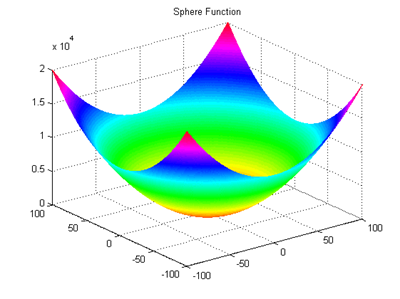
\includegraphics[width=0.6\textwidth]{demo.png}
    \caption{Demo fig}
    \label{fig:demp} 
  \end{figure}
\end{frame}

\section{Float Object Section}

\subsection{Pseudocode}

\begin{frame}
  % \frametitle{Pseudocode} % option frame title
  \begin{algorithm}[H]
  \footnotesize
  \caption{An algorithm with caption}\label{alg:cap}
\KwData{$n \geq 0$}
\KwResult{$y = x^n$}
$y \gets 1$\;
$X \gets x$\;
$N \gets n$\;
\While{$N \neq 0$}{
  \eIf{$N$ is even}{
    $X \gets X \times X$\;
    $N \gets \frac{N}{2}$ \Comment*{This is a comment}
  }{\If{$N$ is odd}{
      $y \gets y \times X$\;
      $N \gets N - 1$\;
    }
  }
}
  \end{algorithm}
\end{frame}

\subsection{Table}
\begin{frame}
  \begin{table}[H]
  \centering
  \begin{tabular}{||c c c c||} 
    \hline
    Col1 & Col2 & Col2 & Col3 \\ [0.5ex] 
    \hline\hline
    1 & 6 & 87837 & 787 \\ 
    2 & 7 & 78 & 5415 \\
    3 & 545 & 778 & 7507 \\
    4 & 545 & 18744 & 7560 \\
    5 & 88 & 788 & 6344 \\ [1ex] 
    \hline
  \end{tabular}
  \caption{Table to test captions and labels.}
  \label{tab:table}
  \end{table}
\end{frame}

\end{document}